\documentclass{standalone}
\usepackage{pgfplots}
\usetikzlibrary{calc}
\usepackage{amsmath}

\begin{document}
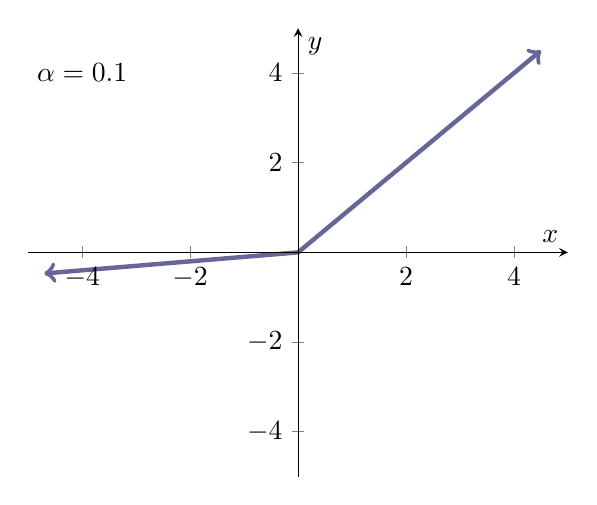
\begin{tikzpicture}

\begin{axis}[
    xmin=-5, xmax=5,
    ymin=-5, ymax=5,
    axis lines=center,
    axis on top=true,
    domain=-4.7:4.5,
    ylabel=$y$,
    xlabel=$x$,
    ]

    \addplot [<->, mark=none,draw=blue!20!gray,ultra thick, samples=500] {(\x<0) * 0.1 * \x + (\x>=0) * \x)};
    
    \node [] at (axis cs:-4,4) {$\alpha = 0.1$};
    
\end{axis}
\end{tikzpicture}
\end{document}